\section{Introduction}
Thus far, the dissertation has focused on perceptual choice. This allowed me to reconcile conflicting findings from other researchers \parencite{spektorWhenGoodLooks2018b,trueblood2013not}. It also allowed me to develop a choice model from the ground up in a simplified choice environment. 

However, many decision theorists, in particular those who study context effects, are interested in a wide variety of choice environments. For example, the original demonstration of the attraction effect came from the marketing literature \parencite{huberAddingAsymmetricallyDominated1982d}, where participants selected amongst hypothetical consumer products. In this chapter, I generalize the paradigm and model from Chapter 2 to consumer choice. Below, I demonstrate results similar to Chapter 2.

\subsection{Expanding the Paradigm to Preferential Choice}

In Experiment 2, I collected psychophysical ratings and used those to estimate the parameters of a Thurstonian choice model, which I then applied to make predictions for choices in the same experiment. To test this approach in preferential choice, it was necessary to collect continuous preference ratings from participants. In Experiment 4, I collected both pricing data (the best continuous measure for consumer stimuli) and choices.

In most studies of consumer preference, researchers collect choice data rather than ratings. There are good reasons for this. The literature on willingness to pay (WTP; the largest amount a given consumer would be willing to pay for a particular product) has shown that, when responding to hypothetical survey questions, participants tend to over-estimate their WTP by a sizeable aomunt \parencite{breidertREVIEWMETHODSMEASURING2006,schmidtAccuratelyMeasuringWillingness2020}, \parencite[c.f.~]{miller2011should}. It is generally more advisable to collect discrete choices, rather than ordinal or continuous ratings, when attempting to measure preferences.

These concerns, while crucial to applied researchers, are not relevant to the current study, as I am interested in participants' relative rather than absolute ratings. In other words, if participants over (or under) estimate their preferences by a constant, but generally rate higher valued options more highly than lower valued options, I can obtain reliable estimates of the $\rho$ parameters. As in Experiment 2, where I was concerned with whether participants' estimates of perceived size increased with absolute size (regardless of how it deviated from actual size), here I am interested in a measure that increases monotonically with the value participants place on each option. 

Other researchers have studied context effects with ratings measures. \textcite{wedellUsingJudgmentsUnderstand} collected Likert scale attractiveness ratings for attraction effect stimuli, generally finding that the presence of a decoy increased mean ratings for a target option. \textcite{windschitl2004dud} asked participants to judge the likelihood of various events (also on a Likert scale). They found that the presence of a "dud" (highly unlikely) alternative increased participants' ratings of focal options. \textcite{caiWhenAlternativeHypotheses2023} and \textcite{fang2024context} demonstrated similar effects by collecting continuous probability judgments.

To my knowledge, however, there has been no research systematically connecting valuations and choices in a single experiment through application of a choice model. Thus, I collected ratings to estimate the multivariate normal parameters $\boldsymbol{\mu}$ and $\boldsymbol{\Sigma}$ for the choice model from Chapter 2 and used these to predict consumer choice data collected from the same group of participants.

\subsection{Correlations in Preferential Choice}
In Chapter 2, I showed that the model could capture the repulsion effect in perceptual choice \parencite{spektorWhenGoodLooks2018b} through target-decoy correlations, estimated via the parameter $\rho_{TD}$. I am now interested in whether 1) preferential choice options also exhibit these correlations and 2) the model can capture the repulsion effect in preferential choice. 

The literature on the repulsion effect in preferential choice is relatively sparse. \textcite{liaoInfluenceDistanceDecoy2021} varied TDD in preferential choice and found a U-shaped relationship between TDD and RST (Relative Share of the Target), with the attraction effect occuring at low and high TDD levels but the repulsion effect occuring at more intermediate TDD levels. 

\textcite{banerjeeFactorsThatPromote2024} demonstrated a binary-ternary form of the repulsion effect using the stimuli depicted in Figure~\ref{fig:banerjee_stim}, across multiple experiment. Participants saw either two or three options on each trial, each varying on two dimensions. The options were consumer choice products from a number of categories (e.g., cameras, coffee makers, laptops), and the dimension names varied by product category (e.g., coffee makers' dimensions were brew speed and features). Attribute values were always displayed numerically using ratings of 1-100.

In each set, the target was always the most extreme option - particularly high on one dimension and particularly low on the other dimension. The competitor was a more intermediate option. For example, consider the blue-colored stimuli in Figure~\ref{fig:banerjee_stim}. $t$ is very high on $X$ and very low on $Y$. Compared to $t$, $c$ is slightly worse on $X$ but slightly better on $Y$. $d$, however, is as high as $t$ on $X$ but even worse on $Y$. 

Using these stimuli and across multiple experiments, \textcite{banerjeeFactorsThatPromote2024} showed that the competitor's choice share increased from binary to ternary choice sets, $P(C|[T,C,D])>P(C|[T,C])$, in violation of the regularity principle \parencite{marley1989random}. In other experiments, they also showed that the repulsion effect decreased with $TDD$.

\begin{figure}
    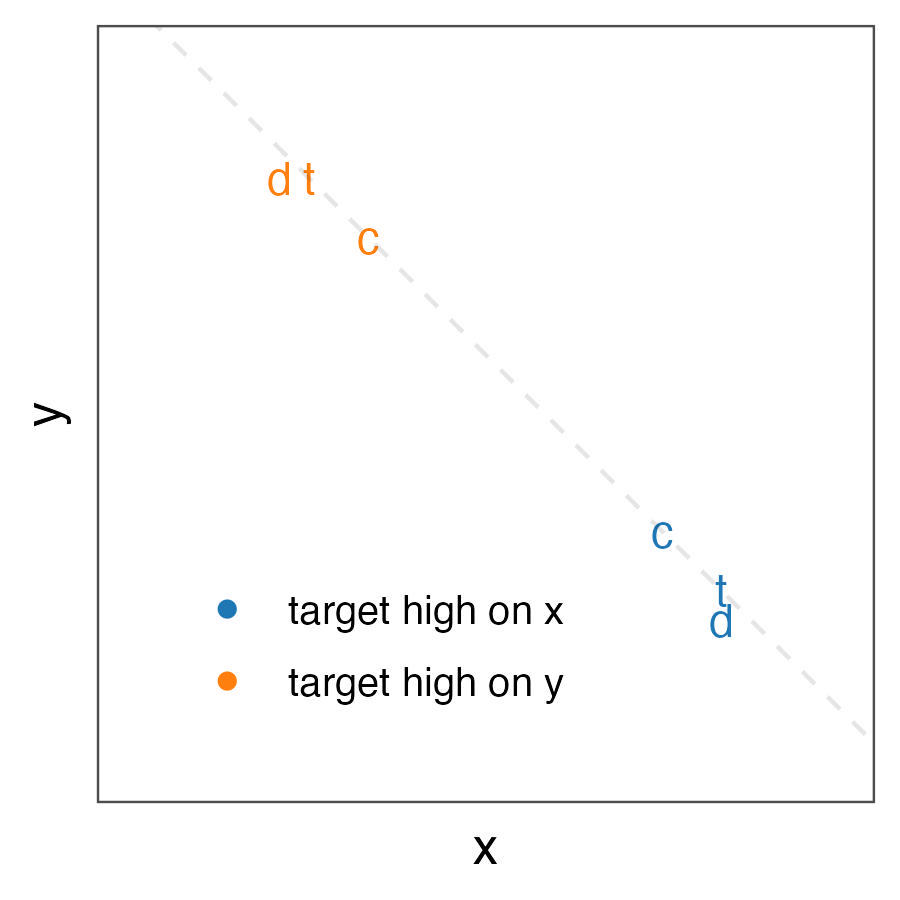
\includegraphics[width=100mm]{figures/banerjee_stim.jpeg}
    \caption{Graphical depiction of a subset of the stimuli used in \textcite{banerjeeFactorsThatPromote2024}, Experiment 5. Target, competitor, and decoy are labeled \textit{t}, \textit{c}, and \textit{d}, respectively. Dimensions are (generically) labeled X and Y.}. The choice sets vary based on whether the target is higher on the X or Y dimension.
    \label{fig:banerjee_stim}
\end{figure}

\textcite{banerjeeFactorsThatPromote2024}'s experiments compared binary to ternary choice rather than ternary to ternary choice, as in \textcite{spektorWhenGoodLooks2018b}. To do a ternary-ternary comparison, one would "flip" the target and competitor labels, such that the target is the intermediate option, the competitor is the extreme option, and the decoy is nearby the new, intermediate target. It is in one sense, quite interesting, that \textcite{banerjeeFactorsThatPromote2024} were able to generate violations of regularity in this binary to ternary comparison. However, the results are somewhat limited by the fact that the target was always more extreme than the competitor.

\textcite{banerjeeFactorsThatPromote2024} argued that their results are consistent with the "tainting hypothesis" \parencite{simonson2014vices} because the repulsion effect is strongest when the target and decoy are similar. They also argued that the decoy, may have caused participants to focus more attention on the competitor's superior dimension. For example, in the blue choice set of Figure~\ref{fig:banerjee_stim}, the decoy is quite poor on $Y$ while being equally good as the target on $X$, so participants may have focused more attention on $Y$, leading to a preference for the target. 

\textcite{banerjeeFactorsThatPromote2024}'s results are interesting and worth exploring further. The authors are also remarkably transparent about their stimulus generation procedure, in addition to posting their data online, so their stimuli were a perfect candidate for the Experiment 4.

\section{Experiment 4}

With Experiment 4, I sought to collect ratings and choice data in a preferential choice setting using (a subset of) \textcite{banerjeeFactorsThatPromote2024}'s Experiment 5 stimuli. I used these data to estimate the parameters of the choice model from Chapter 2. 

For a ratings measure, I asked participants to assign prices to each option. Though people often overestimate prices \parencite{breidertREVIEWMETHODSMEASURING2006}, pricing measures are approximately continuous and monotonic with value and are thus comparable to estimated area (the value measure from Experiment 2).

\subsection{Methods}

\subsubsection{Participants}
137 U.S. adults participated in the experiment. Participants were recruited from Prolific, an online platform for posting research studies, and they were paid $\$5$ for their participation. 24 participants were removed from all analyses for failing catch trials (see below), leaving a final sample size of $N=113$. The mean age was $38.89$ ($SD=11.48$). $61$ participants identified as female, $50$ identified as male, $1$ participant identified as non-binary, and $1$ participant preferred not to say.

\subsubsection{Stimuli}

The stimuli were borrowed from \textcite{banerjeeFactorsThatPromote2024}'s Experiment 1. The stimuli were hypothetical consumer choice products. All stimuli varied on two attributes, each of which ranged from 0-100. The products came from four different categories: televisions, washing machines, laptops, and microwave ovens. 

The attributes varied by category. Televisions varied on screen size and average lifespan. Washing machines varied on average lifespan and energy savings. Laptops varied on processing speed and memory (RAM). Microwave ovens varied on warranty and cooking power. 

Within each category, one attribute was arbitrarily designated as dimension 1 and another as dimension 2 (see below). 

\subsubsection{Design}

The experiment took place in two phases: pricing and choice. The trial types were identical for both phases.

In each phase, there were two types of trials: critical trials and catch trials. The critical trial stimuli are shown in Figure~\ref{fig:ce_rating_stim}. 

There were two types of critical trials: those designed to elicit the repulsion effect (a replication of \citeauthor{banerjeeFactorsThatPromote2024}), and those designed to elicit the attraction effect. Within both the attraction and repulsion trials, I varied which dimension the target was higher on (1 or 2), $TDD$ (designated near or far), and product category (microwaves, washing machines, laptops, and televisions). Note that to create the attraction trials, I simply "shifted" the target and competitor towards the center of the attribute space. That is, target and competitor are equally similar in both repulsion and attraction trials, but they are both more extreme in the repulsion trials.

\begin{figure}
    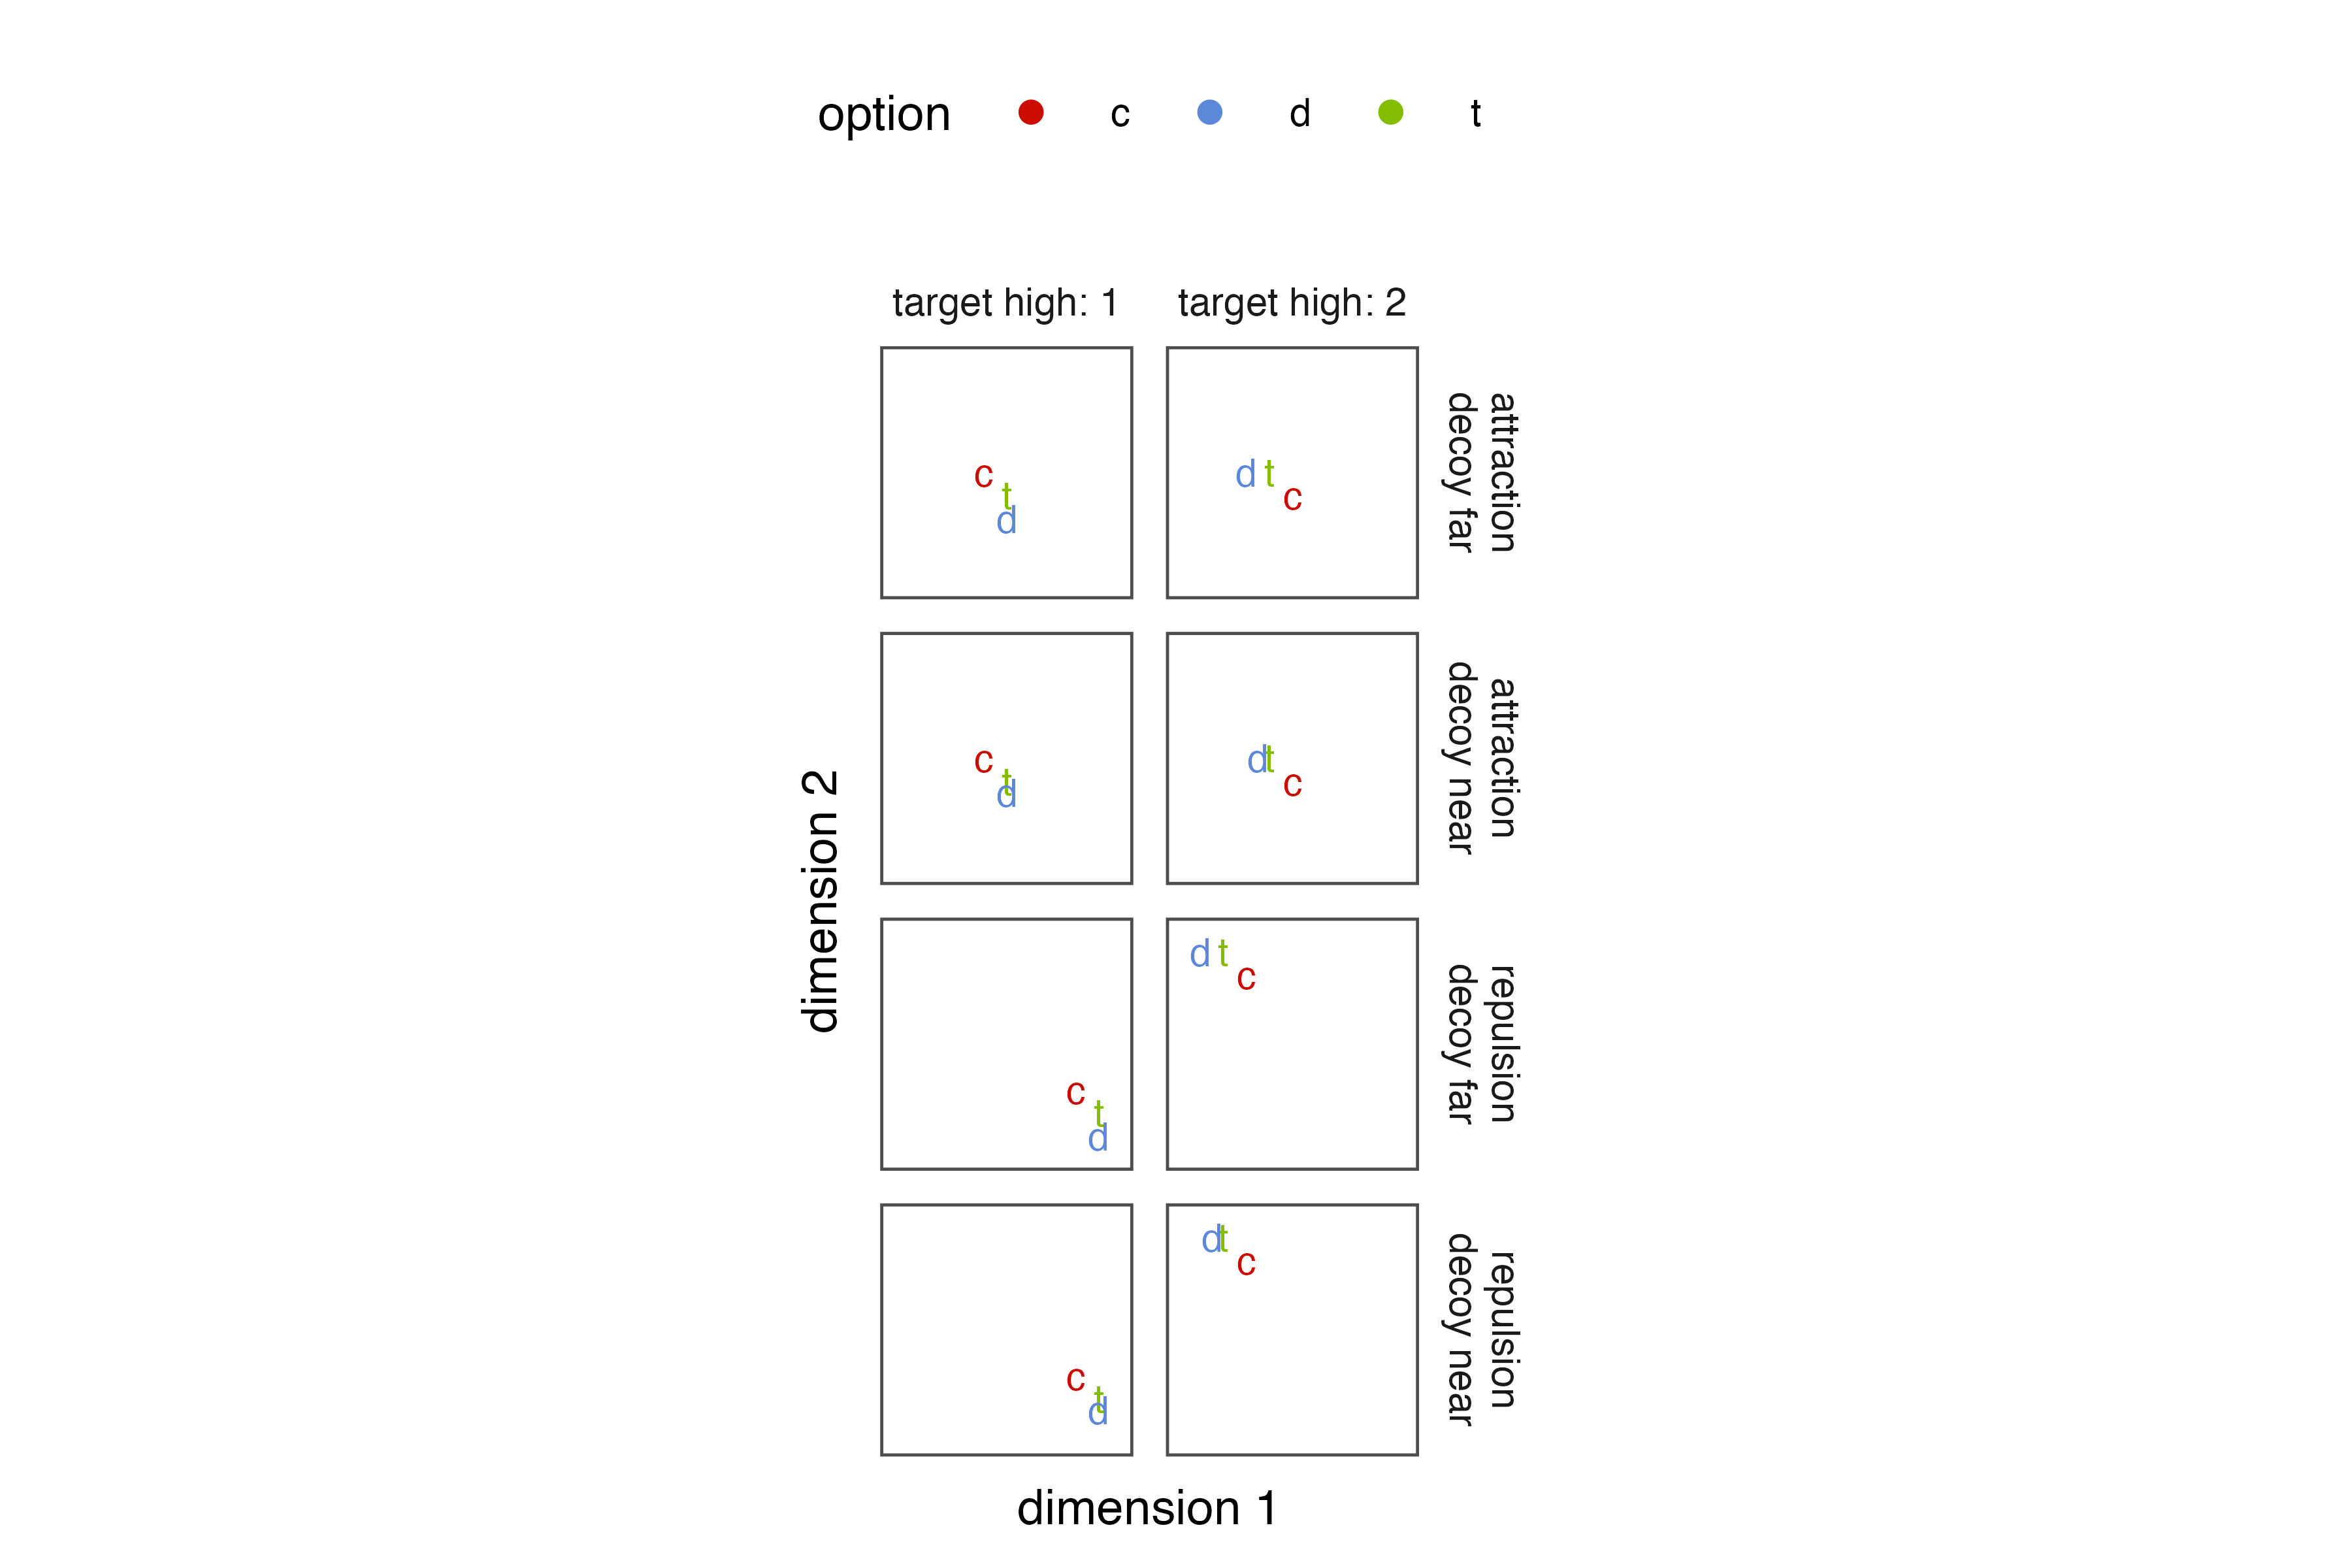
\includegraphics[width=150mm,scale=0.5]{figures/ce_rating_stim_for_paper.jpeg}
    \caption{Graphical depiction of the critical stimuli from Experiment 4. Rows show the different choice sets designed to elicit the attraction/repulsion effect, with the label also specifying whether the decoy is near or far from the target in attribute space. The columns indicate which dimension the target is high on (1 or 2).}
    \label{fig:ce_rating_stim}
\end{figure}

The catch trials were designed such that one option was clearly superior to the other two. On each catch trial, the superior option's dimension values were each randomly sampled from the distribution $U(50,95)$, while the two inferior option's dimension values were sampled from the distribution $U(5,50)$. All dimension values were rounded to multiples of 5. 

In each phase, there were 32 critical trials (16 designed to elicit the repulsion effect and 16 designed to elicit the attraction effect) and 8 catch trials.

I did not test binary repulsion effect trials, as in \textcite{banerjeeFactorsThatPromote2024}'s experiments, so I cannot assess the repulsion effect to the same degree as those authors. The goals here are, rather, to measure valuation correlations in consumer preference and attempt to relate them to choice.

\subsubsection{Procedure}

The experiment took place in two phases: a pricing phase and a choice phase.

Prior to the pricing phase, participants were provided with a cover story. According to the cover story, they were told to imagine that they run an online consumer goods resale business. On each trial, they would see three products, and they needed to determine which price to sell each product for. Participants were also told that they should determine a price that maximizes both profit and the likelihood the product is purchased. 

During the pricing trials, the three options were presented in a table, with the options in rows and the attributes in columns. All attributes were represented numerically. The options were labeled A, B, and C. The last column of the table contained three boxes, which participants used to type in their selling price for each option. Participants typed in their selling price, and then clicked a button on screen to move onto the next trial. Both option order and dimension order was randomized on each trial. See Figure~\ref{fig:ce_rating_choice_trial} (left panel) for an example trial. Participants were only allowed to enter in whole numbers (e.g., dollars not cents).

\begin{figure}
    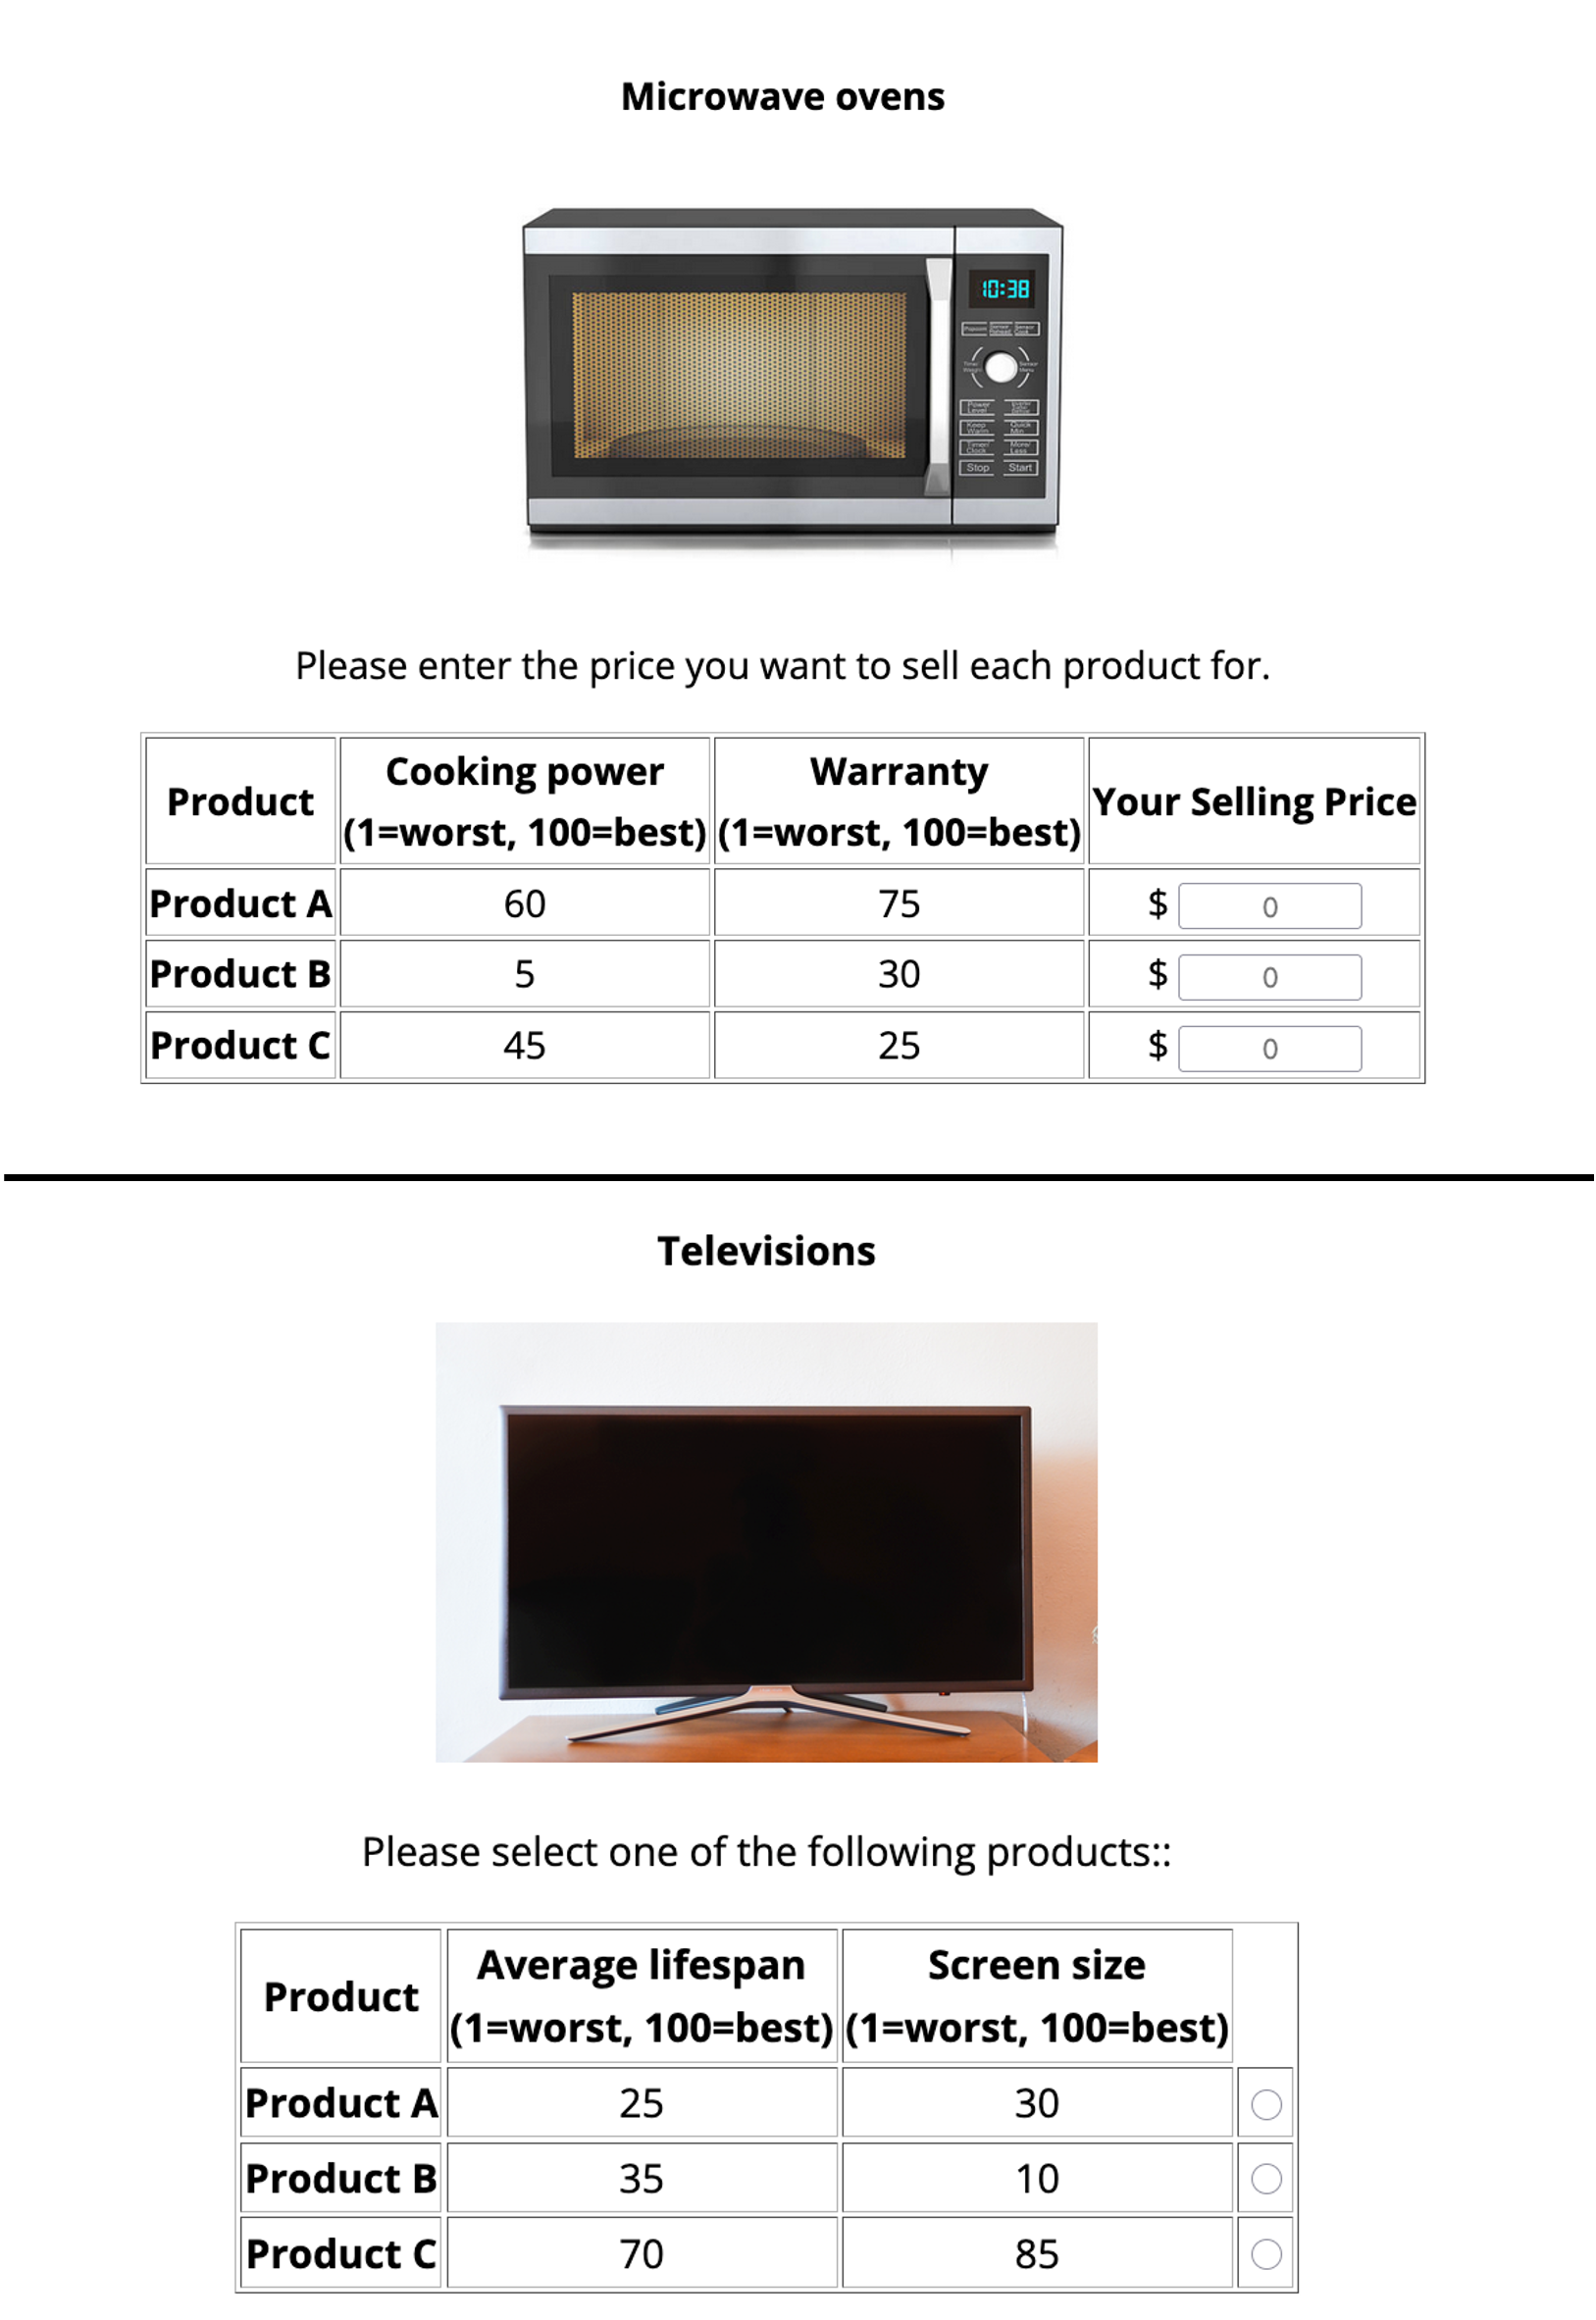
\includegraphics{figures/ce_rating_choice_example_trial.jpg}
    \caption{Sample trials from the pricing phase (top) and choice phase (bottom) in Experiment 4.}
    \label{fig:ce_rating_choice_trial}
\end{figure}

After completing all pricing trials, participants moved onto the choice phase. Prior to this phase, participants were told to imagine that they were purchasing consumer goods in bulk. On each trial, they were to select the option they wanted to purchase. 

As in the pricing phase, options were presented in a table, where option order and dimension order was randomized. See Figure~\ref{fig:ce_rating_choice_trial} (bottom) for an example trial.

After the choice phase, participants completed a short demographics form.

\subsection{Results}

\subsubsection{Data Processing}

First, I removed 24 participants who did not pass at least $5/8$ catch trials in both the pricing phase and the choice phase. To pass a pricing catch trial, the participant needed to price the superior option at least as high as the other two, inferior options. To pass a choice catch trial, the participant needed to select the superior option. 

\subsubsection{Pricing Trials}

First, I computed mean prices for the target, competitor, and decoy option within each trial type and product category. These means are shown in Figure~\ref{fig:price_m_by_effect_category}.

On average, participants priced the target and competitor higher than the decoy. They also assigned higher prices to products that are typically more expensive (e.g., washing machines are more expensive than microwave ovens). This suggests that participants were engaged with the task and, in a relative sense, performed the task well.

\begin{figure}
    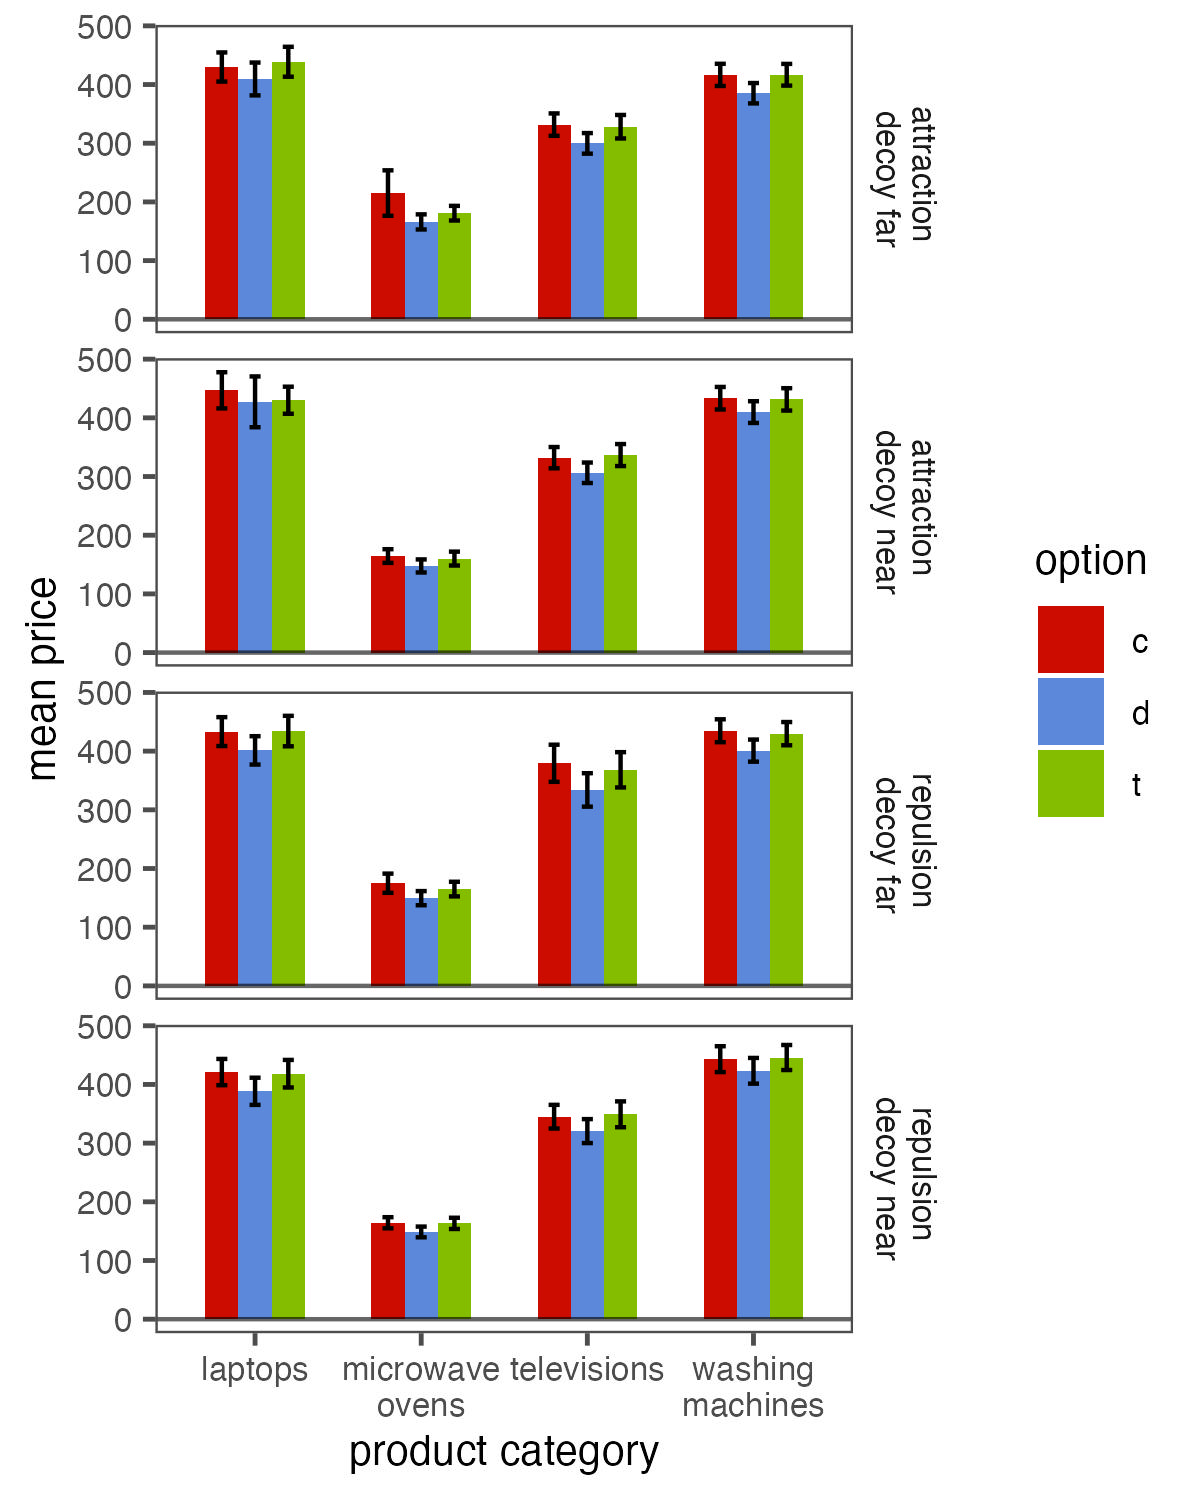
\includegraphics[width=200mm,scale=0.5]{figures/price_m_by_effect_category.jpeg}
    \caption{Experiment 4 mean prices by product category, option, and trial type. Error bars are $\pm 1\;\text{SEM}$.}
    \label{fig:price_m_by_effect_category}
\end{figure}

I performed a Bayesian modeling analysis comparable to that of Experiment 2. I estimated the mean prices and the correlations between prices. These results can be found in the Appendix. Below, I discuss descriptive statistics, but whenever I claim that one parameter value is greater than another, the reader can see the Appendix to support these conclusions. The ordering of these correlations, however, is the same in both the model-based and the descriptive analysis.

% Additionally, I report the descriptive values for all correlations, rather than those based on model estimates, as the latter as biased downard due to limited data \parencite{stephens2020state,merkle2023opaque}. 
To account for participant-level differences in pricing, I first z-scored all prices within each participant. To avoid the influence of outliers on correlation estimates, I removed trials in which at least one z-score had an absolute value $>3$. 

I computed the mean prices for target, competitor, and decoy options within each trial type, collapsing over product category and TDD, in Figure~\ref{fig:price_mu_model_data}. In both repulsion and attraction effect trials, the target and competitor do not differ in mean price, while both are priced higher than the decoy option.

\begin{figure}
    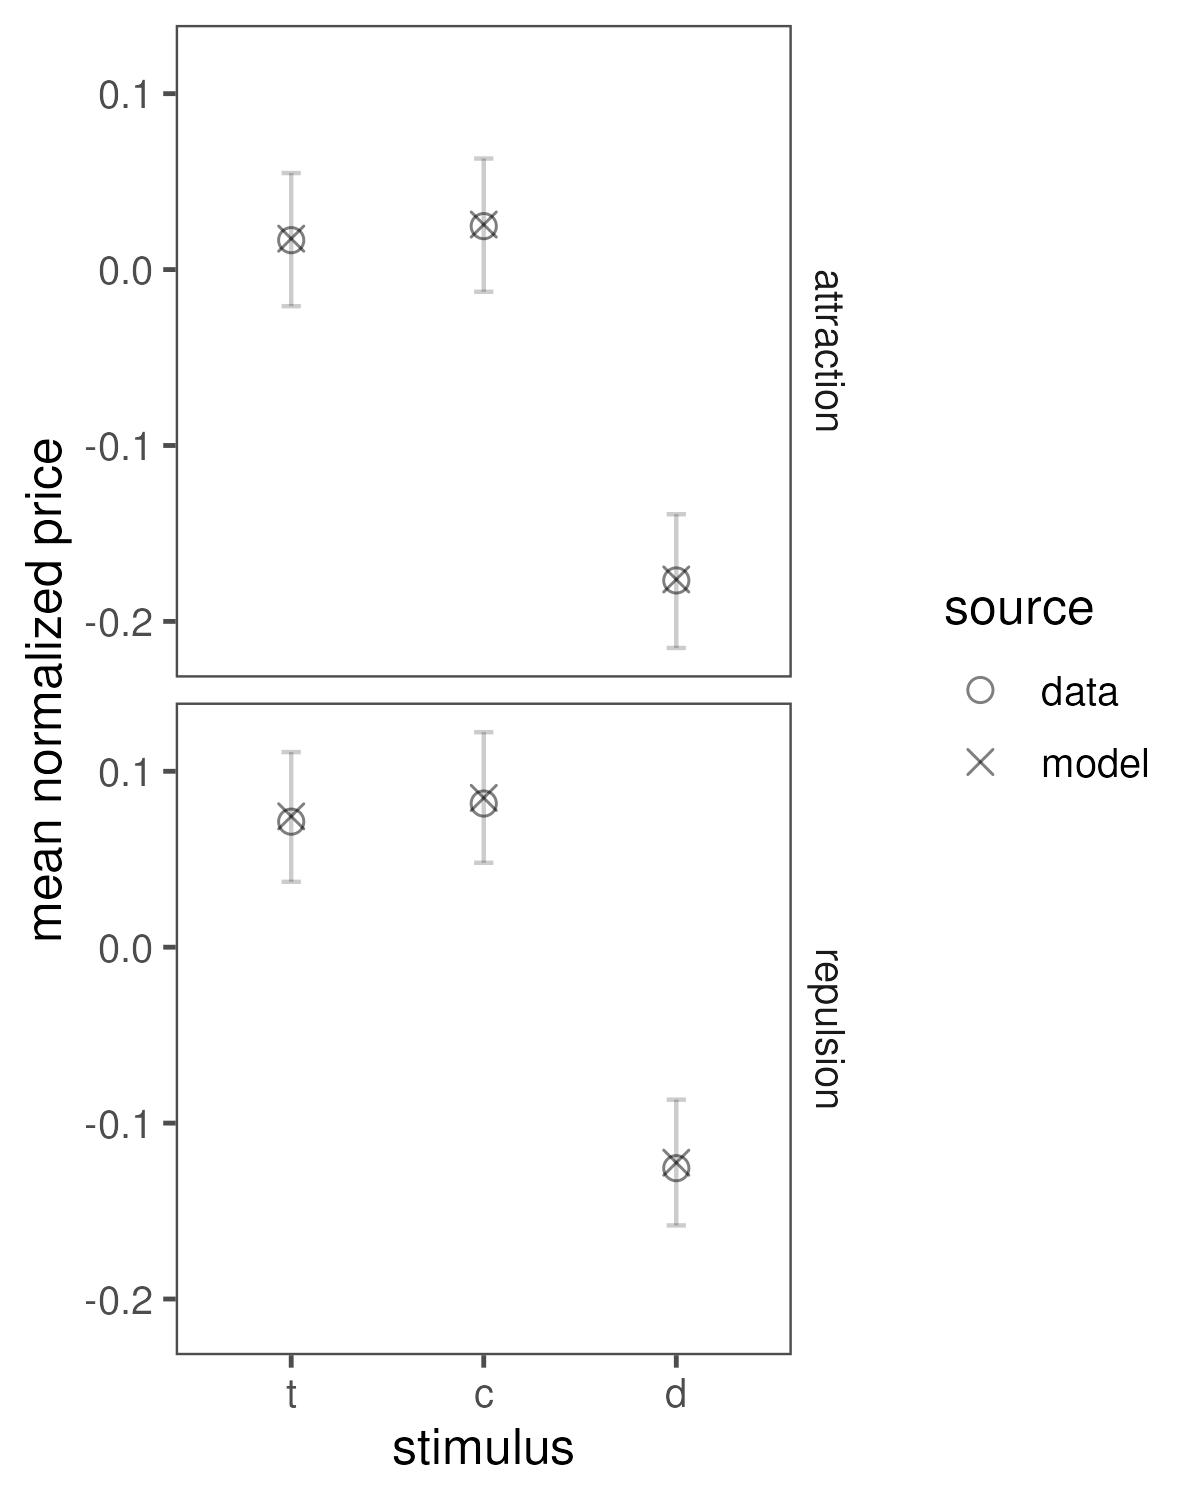
\includegraphics[scale=0.5, width=100mm]{figures/pricing_mu_model_data.jpeg}
    \caption{Experiment 4 mean prices for target, competitor, and decoy options in both repulsion and attraction trials. Model values are the means from the posterior distribution, and error bars are $95\%$ HDIs.}
    \label{fig:price_mu_model_data}
\end{figure}

I then computed correlations between the prices assigned to options within each trial type. I plot the z-scored prices in a series of scatterplots, with the Pearson correlations included. See Figure~\ref{fig:price_z_corplot_repulsion} for repulsion effect correlations and Figure~\ref{fig:price_z_corplot_attraction} for attraction effect correlations. 

In the repulsion trials, I replicated the results of Experiment 2, in that $\rho_{TD}>\rho_{TC}$ and $\rho_{TD}>\rho_{CD}$. Interestingly, I also found that $\rho_{TC}>\rho_{CD}$, while in Experiment 2 $\rho_{TC}\approx\rho_{CD}$.

In the attraction trials, I found that $\rho_{TC}>\rho_{TD}>\rho_{CD}$. In other words, the target and competitor are more similar than target and decoy, which are in turn more similar than competitor and decoy. 

\begin{figure}
    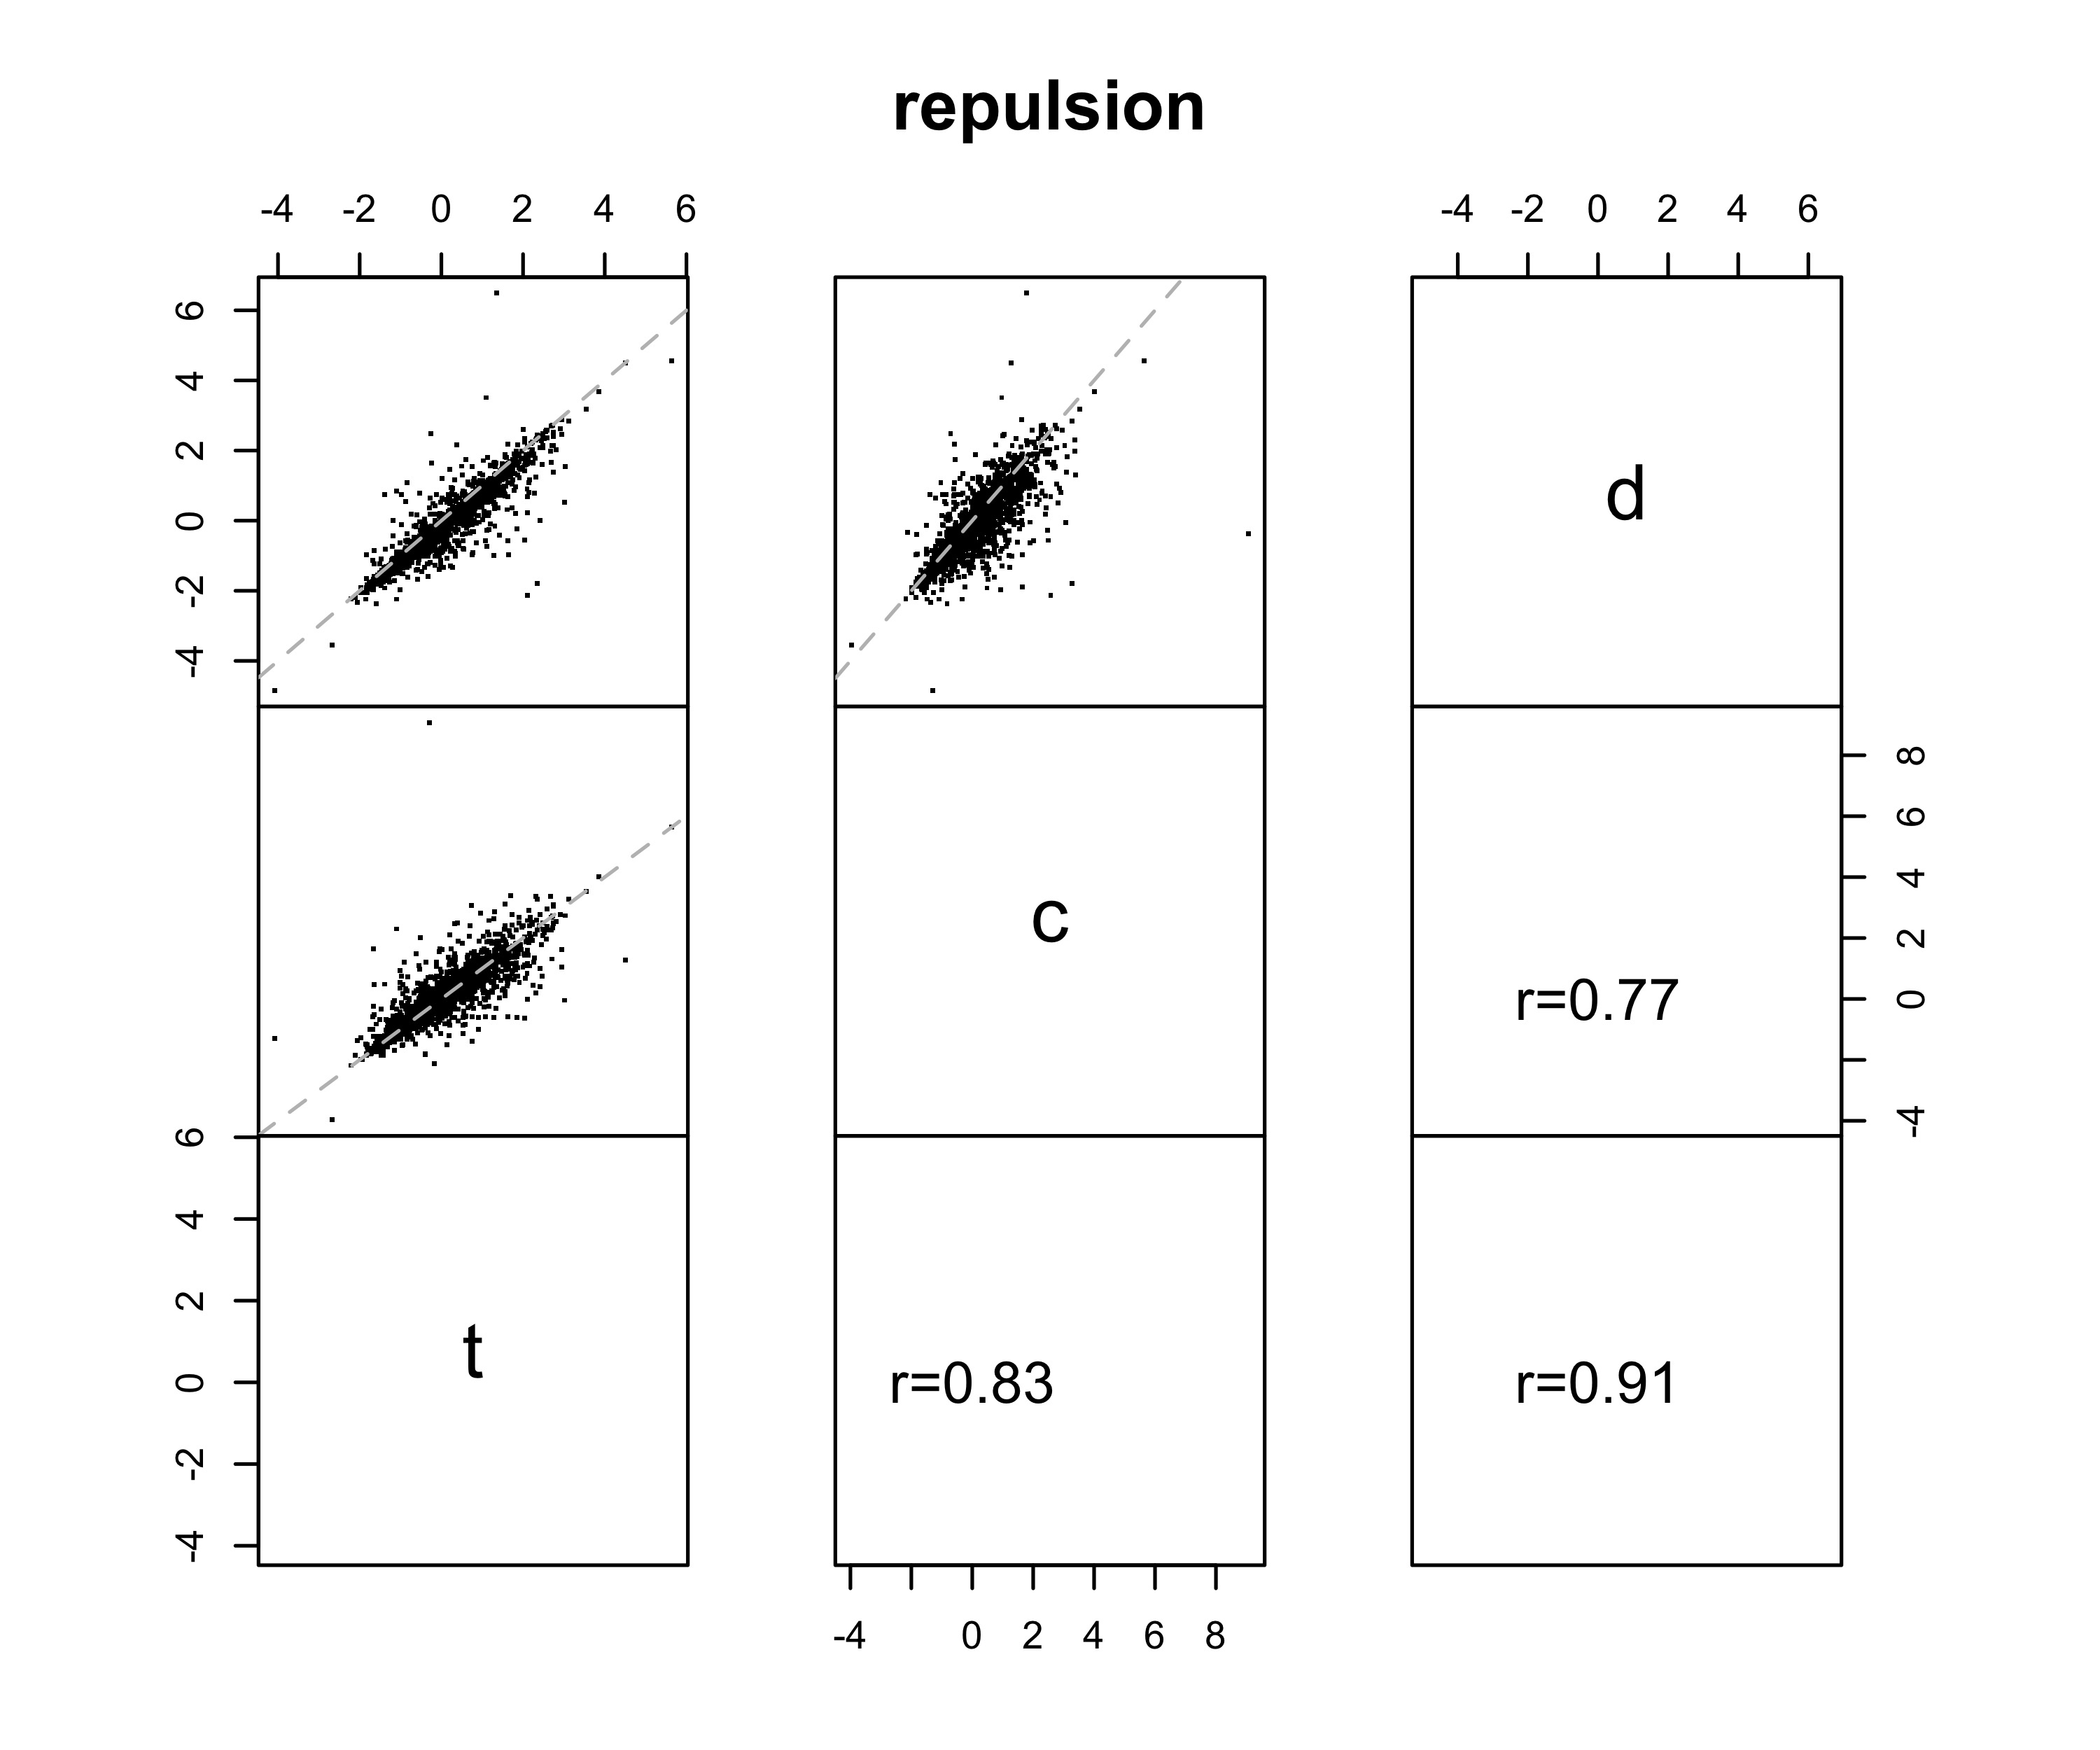
\includegraphics[scale=.5,width=120mm]{figures/price_z_corplot_repulsion.jpeg}
    \caption{Experiment 4 correlation plots for all pairs of stimuli, in trials designed to elicit the repulsion effect. t=target, c=competitor, and d=decoy.}
    \label{fig:price_z_corplot_repulsion}
\end{figure}

\begin{figure}
    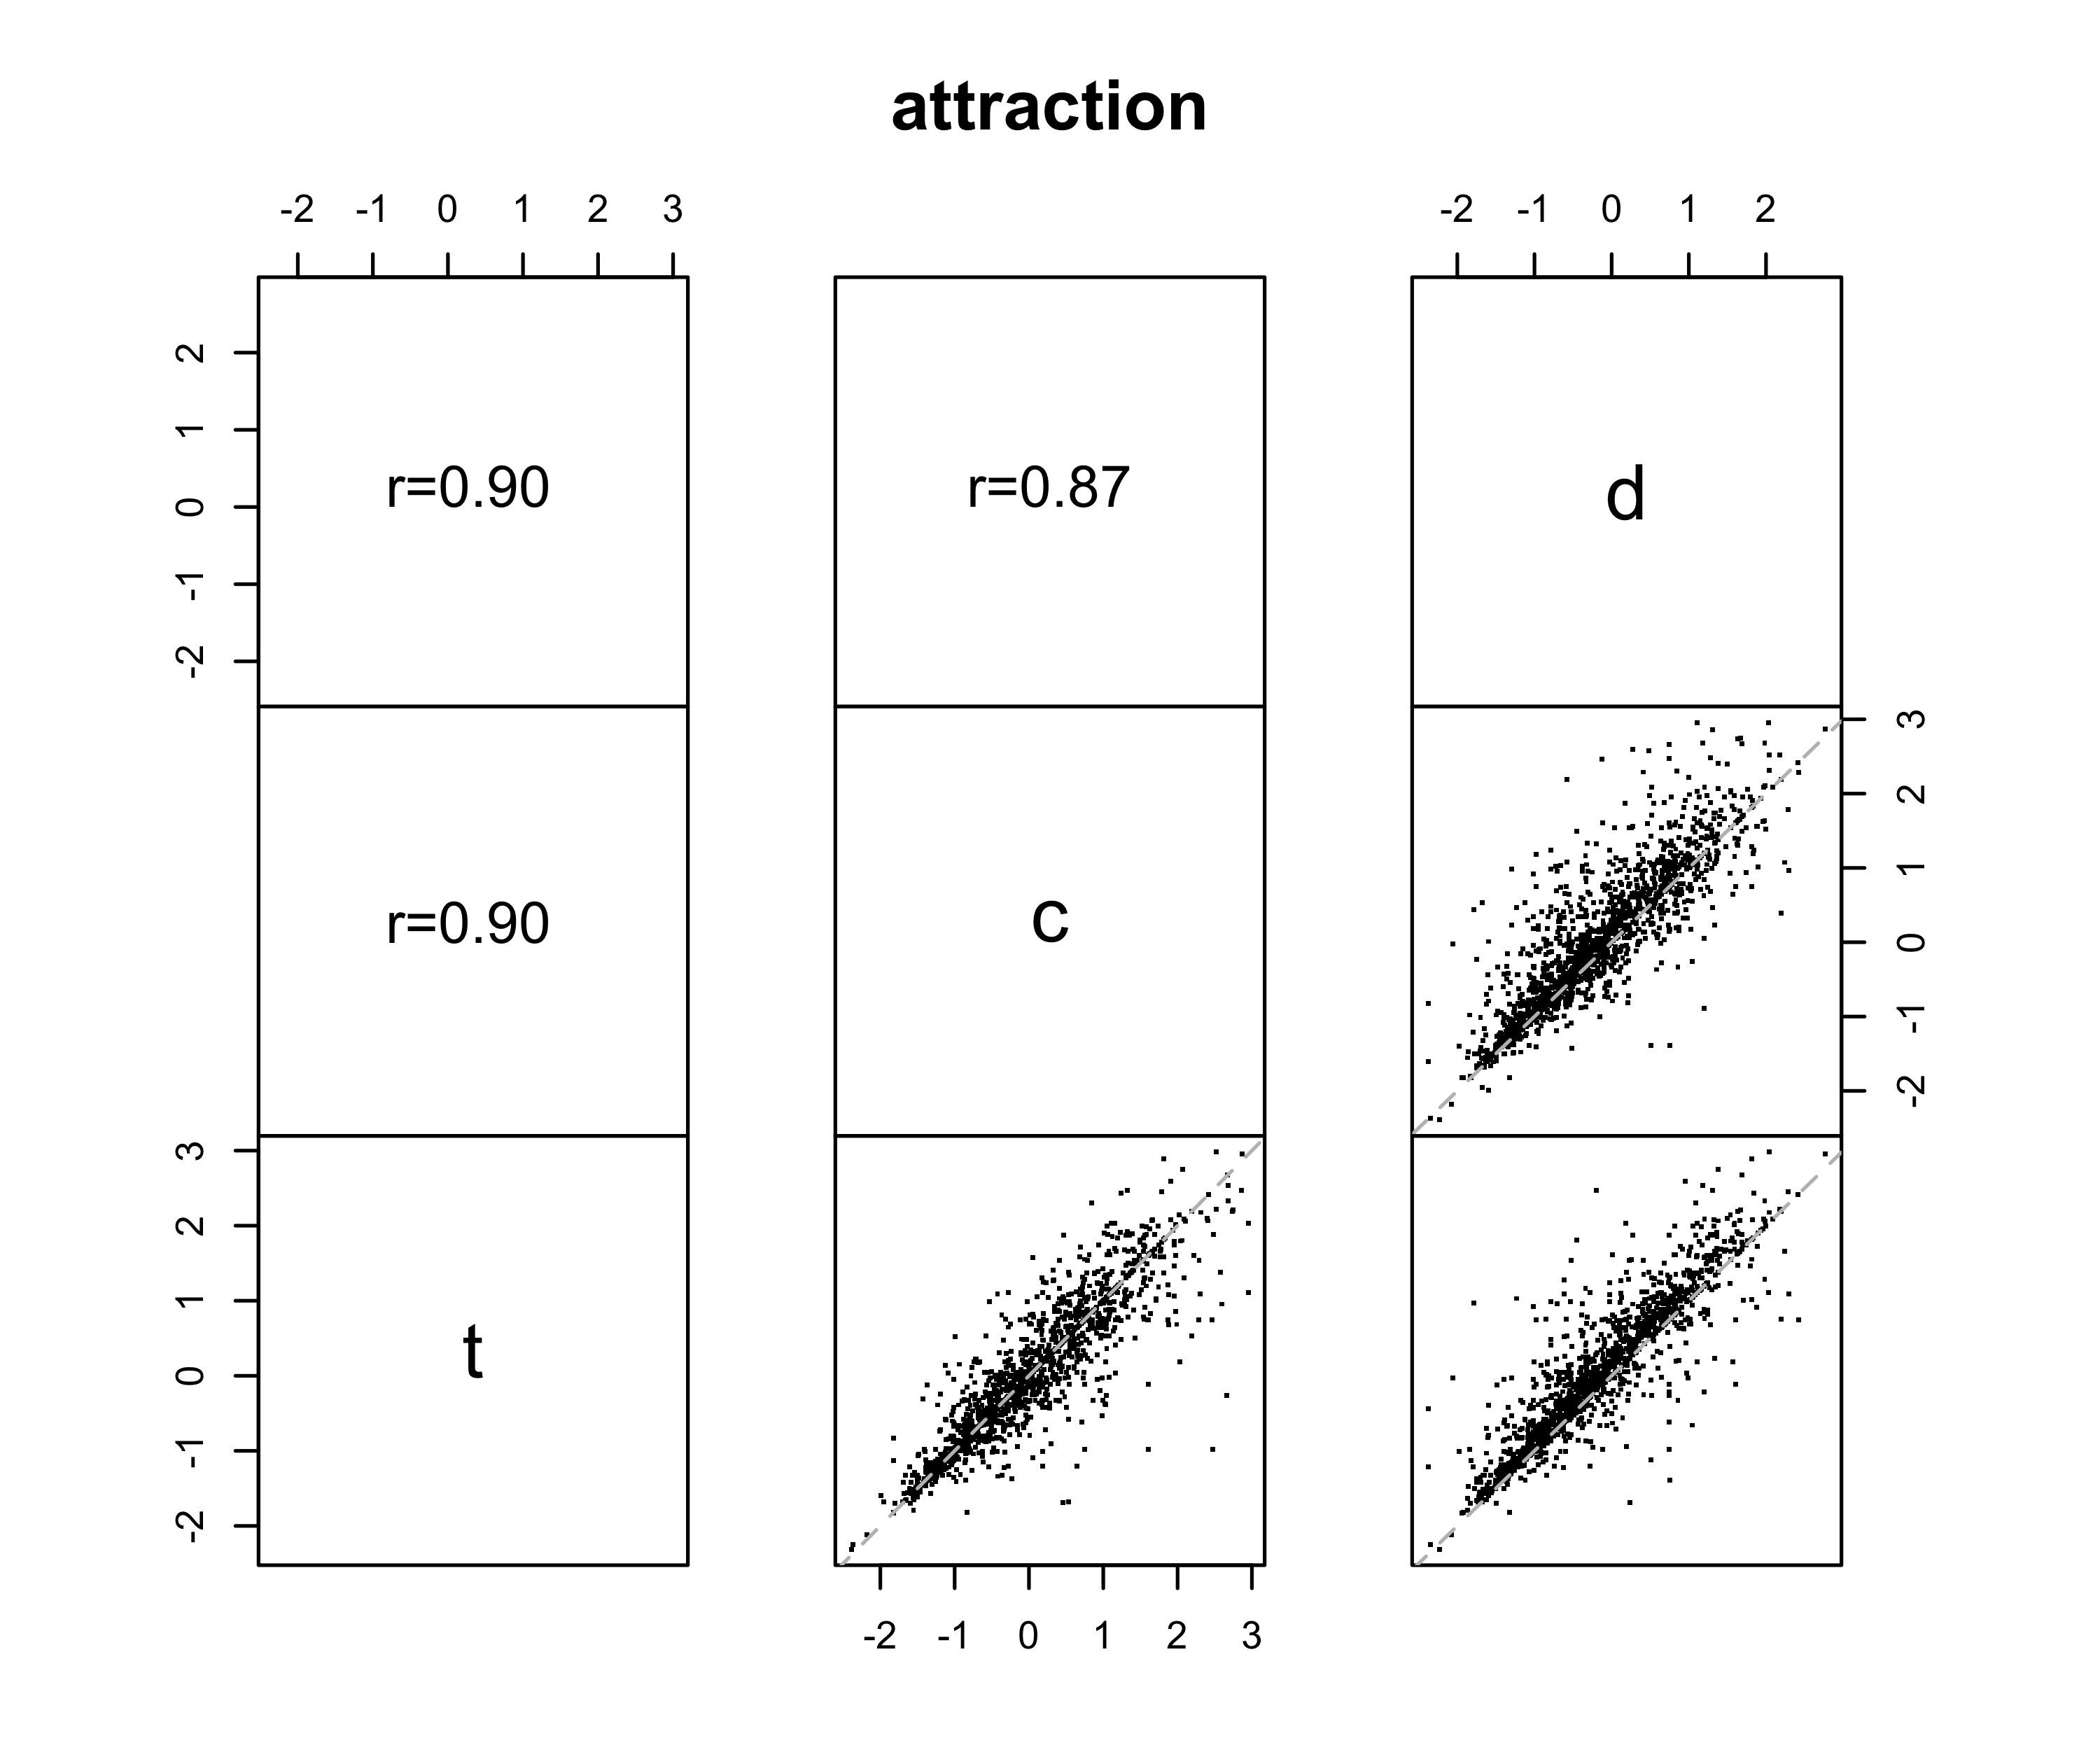
\includegraphics[scale=.5,width=120mm]{figures/price_z_corplot_attraction.jpeg}
    \caption{Experiment 4 correlation plots for all pairs of stimuli, in trials designed to elicit the attraction effect. t=target, c=competitor, and d=decoy.}
    \label{fig:price_z_corplot_attraction}
\end{figure}

\subsubsection{Choice Trials}

I next computed choice proportions for the critical choice trials. I collapsed across participant (due to the small $n$ per subject), as well as product category and the target's superior dimension.

These choice proportions are plotted in Figure~\ref{fig:bayes_choice_model_data_plot}. The results clearly show a null attraction effect, regardless of $TDD$. Participants chose the target and competitor options at equal rates. This is likely due to the strong similarity of target and competitor, atypical of attraction effect studies. 

The results show what appears to be a repulsion effect, where the participants generally prefer the competitor option to the target option. However, because I did not include a ternary-ternary comparison (i.e., varying whether the decoy is located nearer to the extreme option or to the intermediate option), these results may be due to participants simply preferring the less extreme option.

Participants seldom chose the decoy, another indication that they were attentive to the task. This also provides evidence that decoy selection is far more common in perceptual choice than preferential choice.

\begin{figure}
    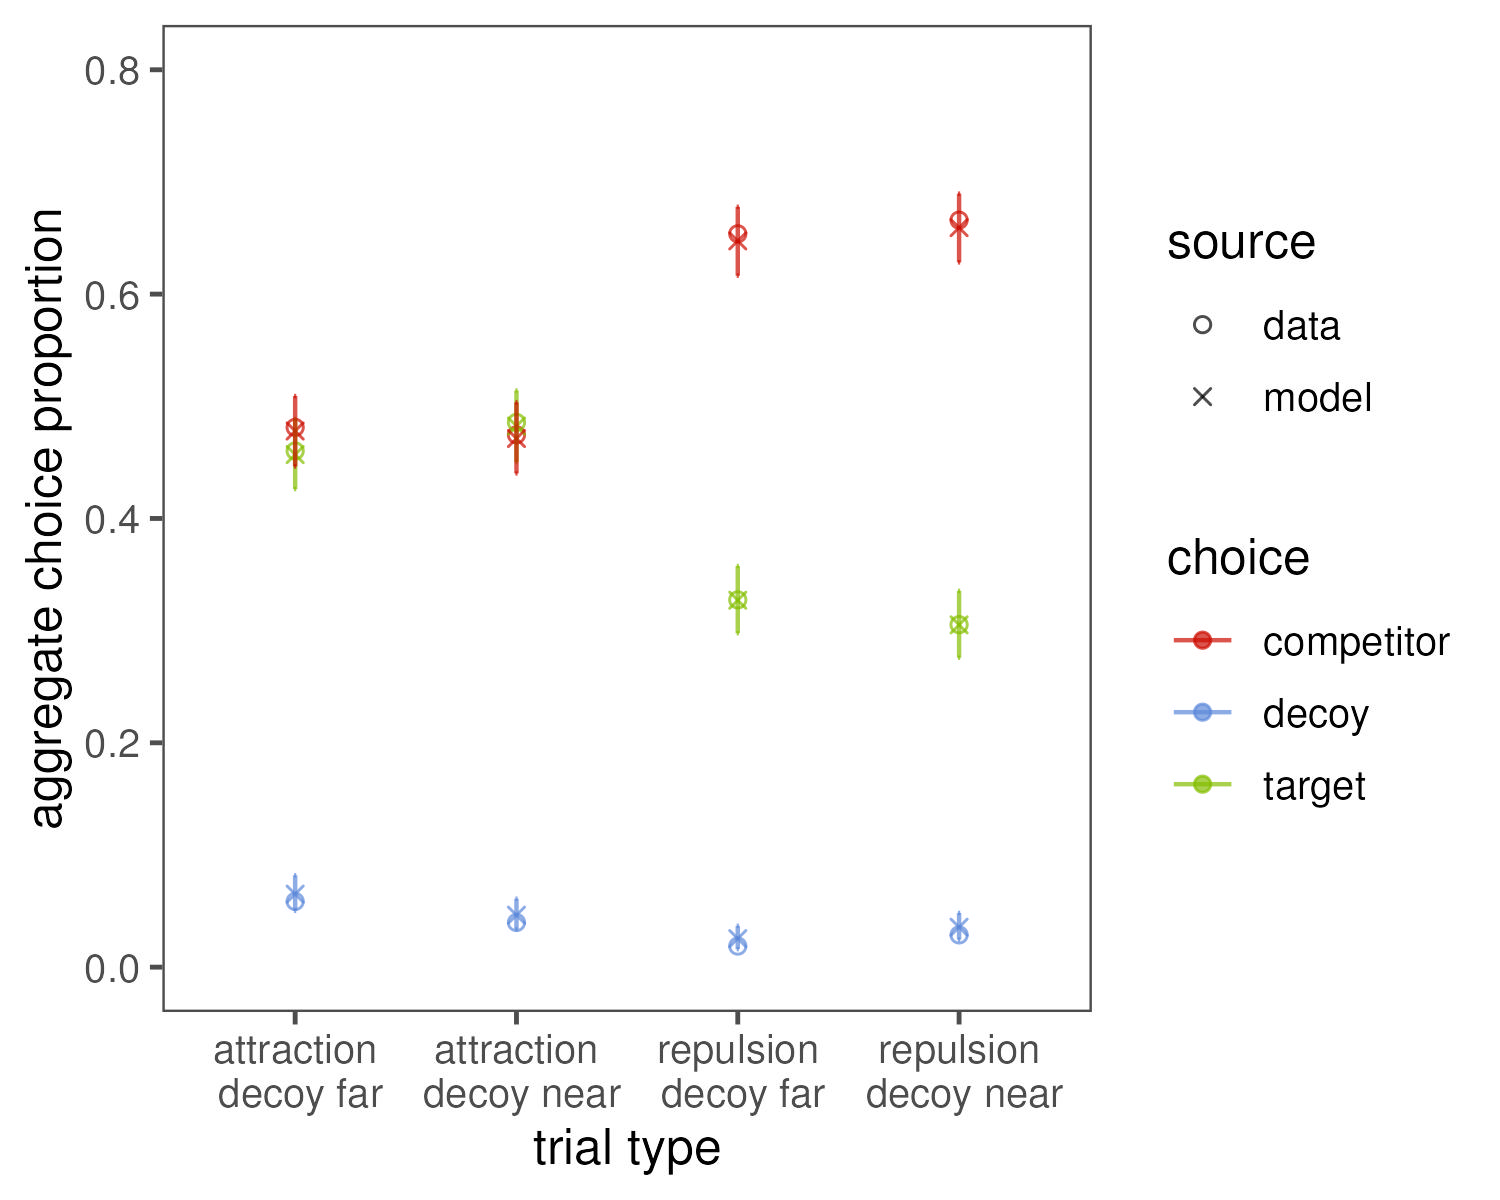
\includegraphics[scale=.5,width=100mm]{figures/bayes_choice_model_data_plot.jpeg}
    \caption{Experiment 4 aggregate choice proportions for each trial type, TDD, and option. Data points are aggregate choice proportions, while model points are posterior means computed from the Bayesian Dirichlet-multinomial model presented in the Appendix. Error bars are $95\%$ HDIs.}
    \label{fig:bayes_choice_model_data_plot}
\end{figure}

\subsubsection{Model Simulations}

As in Chapter 2, I used the parameter estimates for $\boldsymbol{\mu}$ and $\boldsymbol{\Sigma}$ to simulate choice. I use the Thurstonian model from Chapter 2, originally used to simulate perceptual choice. 

To simplify this analysis, I only consider attraction and repulsion trials, collapsing over all other factors. 

As in Chapter 2, the model assumes that value is stochastic while choice is deterministic\footnote{This also assumes ties are not possible, which is true if and only if perceived area is absolutely continuous.}. The model always chooses the option perceived as most valuable, regardless of the magnitude of the difference between the "winner" and "runners-up". That is, given a vector $\mathbf{X}_i$ of perceived values on trial $i$ with set $K$, the probability a participant selects stimulus $j$ is:

\begin{align}
   P(j|i,K)=P(\mathbf{X}_{ij}>\mathbf{X}_{ik}), \forall k \in K, j \neq k
   \label{eqn:pchoice_price}
\end{align}

I ran $1,000,000$ simulations of the model and plotted the results against the data in Figure~\ref{fig:bayes_choice_sim_preds}.

\begin{figure}
    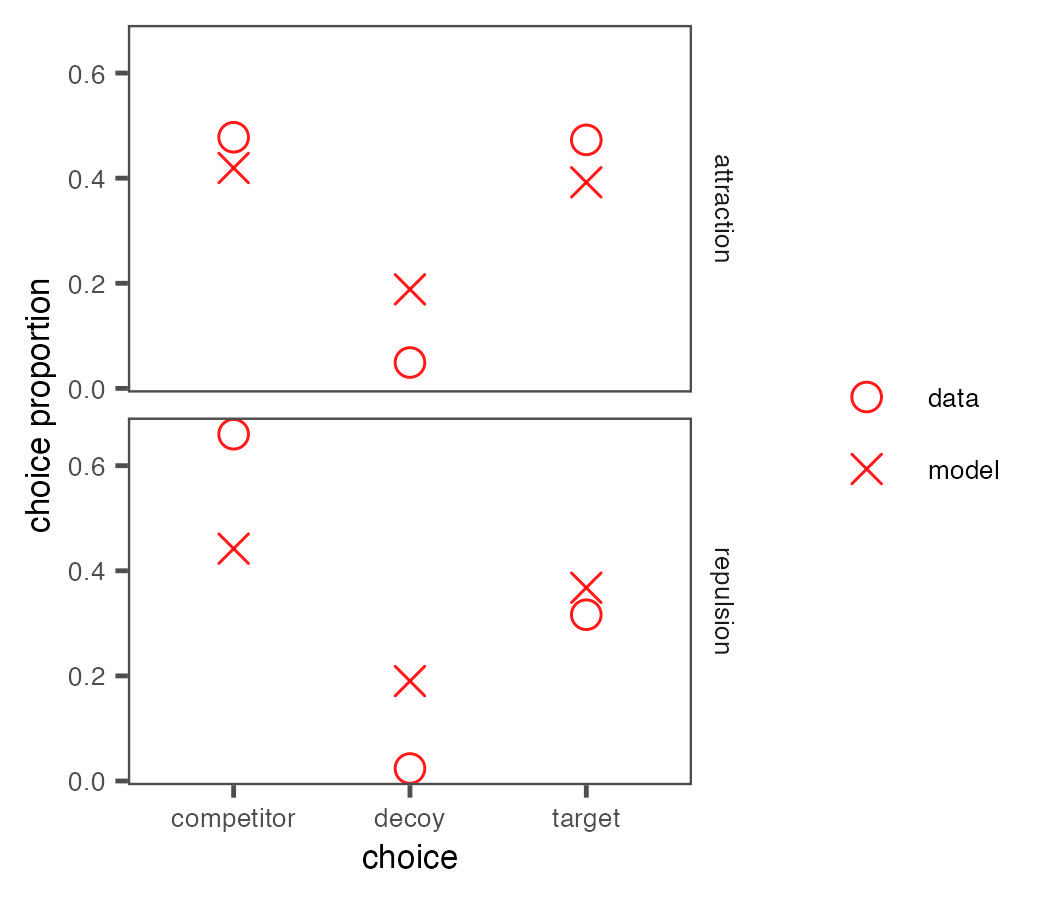
\includegraphics[scale=.5,width=100mm]{figures/bayes_choice_sim_preds.jpeg}
    \caption{Experiment 4 data vs. Thurstonian model predictions.}
    \label{fig:bayes_choice_sim_preds}
\end{figure}

The model mispredicts the attraction trials. It predicts a slight repulsion effect when in fact the data suggest a null effect.

The model successfully predicts a qualitative repulsion effect, i.e., $P(C)>P(T)$. However, it strongly overpredicts decoy choice proportions. The model relies on the correlation between target and decoy choice proportions to predict the repulsion effect. According to the model because the target and decoy are strongly correlated, it is more likely that the utility of the decoy exceeds the target than the competitor. The decoy then "steals" choice shares from the competitor. This prediction makes sense in perceptual choice, where stimulus discriminability is not a given and participants pick the decoy roughly $20$-$30\%$ of all trials (see Experiment 2). In preferential choice, participants almost never pick the decoy, and researchers assume that any participant with sufficient attention can always discriminate the target and competitor from the decoy. Thus, though the model can qualitatively predict a repulsion effect, the mechanism by which it does so is implausible.

\section{Discussion}

This experiment generalizes the paradigm of Chapter 2 to preferential choice. Participants completed two phases; in the first phase, they assigned a selling price to each of three options on each trial. In the second phase, they selected the option they would most prefer. Option sets were designed to either elicit the attraction effect or the repulsion effect. I used the prices to estimate the mean value of each option as well as the correlations between all pairs of options. In doing so, I extended not only the experimental paradigm of Chapter 2, but also the modeling framework, to a preferential choice setting.

Crucially, when estimating the correlations, I replicated the result of Experiment 2, that, in the repulsion effect $\rho_{TD}>\rho_{TC}$ and $\rho_{TD}>\rho_{CD}$. Interestingly, the inferential statistics also show that $\rho_{TC}>\rho_{CD}$. This result was unexpected, but it may be due to the fact that, because both are high on one dimension and low on another, it is easier to compare target and competitor to one another than it is to compare the competitor to the decoy. 

Interestingly, in the trials designed to elicit the attraction effect, I found that $\rho_{TC}>\rho_{TD}>\rho_{CD}$. This is likely due to the similarity of target and competitor on both attributes (i.e., one option's dimension values were $[50,60]$ while the other's was $[60,50]$). The target and competitor are easily comparable to one another, and the tradeoff on attributes is negligible.

The choice results replicated those of \textcite{banerjeeFactorsThatPromote2024}, in that participants chose the competitor more than the target in each of the repulsion effect choice sets. However, given that I did not vary the decoy location (i.e., the competitor was always less extreme than the target), nor did I include a binary-ternary choice comparison. These results may be due to a bias for the less extreme option, which happens to be the competitor in this case. Future research should include binary-ternary and ternary-ternary trials to generalize these results.

The strong correlation between target and decoy valuations appears to be a robust finding, holding across perceptual and preferential choice. It is worth exploring, in greater detail, what causes these correlations. 

In the attraction and repulsion effect, the target and decoy are designed such to be more similar to each other than either option is to the competitor. It may be that, by measuring the correlation in valuations, we are actually measuring the \textit{similarity} between options. Indeed, the similarity of target and decoy was a primary motivation for the original demonstration of the attraction effect \parencite{huberAddingAsymmetricallyDominated1982d}. 

These correlations may also be measuring the ease of comparability between pairs of options. Comparability has previously been shown to drive the attraction effect \parencite{noguchi2014attraction,cataldoComparisonProcessAccount2019b}, and several models of context effects rely on comparisons of options on single attributes to generate context effects \parencite{trueblood2014multiattribute,roeMultialternativeDecisionField2001a}. Supporting this hypothesis is the finding that $\rho_{TC}>\rho_{TD}$ in the trials designed to elicit the attraction effect, when the target and competitor were quite similar on each attribute and thus easier to compare.

Future work could test these hypotheses by systematically manipulating option comparability and assessing whether the correlations vary with comparability. I work towards this in Chapter 5 through testing the effect of comparability on choice, but it would be interesting to directly measure correlations in choice environments of varying comparability. 
